\chapter{Implementation}
\label{ch:implementation}
From a practical point of view, the aim of this project was to create a working web application that also makes use of the best available development practices, well-designed architecture and is easy to maintain and extend in the future. The application is a relatively small-scale one, but it was developed with a future large-scale application in mind, that would support a large number of concurrent requests and stay highly responsive. Therefore, great emphasis was put on the scalability and performance.  

This chapter examines the process of the application development. 

\section{Choice of Technologies}
\label{sec:choiceoftechnologies}
The application will be built using a set of front end and back end technologies. In this section will be justified the choice made in favour of each particular technology used in the project. 

\subsection{Front End}
\label{subsec:frontend}
The markup of the future application will be coded using HTML 5 \citep{documentation:HTML}. The application markup will be built using BEM front end development approach \citep{documentation:BEM}. BEM (short for "Block Element Modifier") is a popular semantic model for markup and a way to organise sections of a website into purposeful blocks and to optimise CSS. The idea behind is to logically break the HTML down into \emph{independent} blocks, which will allow arbitrary placement of the block anywhere on the page, including nesting the block inside another block. The approach can be  very beneficial for large websites, allowing the code to be reused across pages or even projects. However, a small project like the SureThing can also benefit from BEM by making use of independent, context-free CSS that can be easily amended in the future \citep{article:BEMForSmallProjects}.

CSS3 is used to define the visual presentation of the application. In general, CSS has certain limitations of its syntax capabilities. For example, it does not allow the use of variables, macros, mixins (reusable blocks of styles) functions and other features associated with object-oriented development, which inevitably leads to the creation of immensely repetitive stylesheets. In order to overcome those limitations, SASS preprocessor \citep{documentation:sass} will be used in this project. SASS (short for Syntactically Awesome Stylesheets) is a powerful language that extends CSS with a choice of useful functionality, all in CSS-compatible syntax. Use of SASS would allow to make CSS code more efficient and easily maintainable. 

In addition to that, SureThing will make use of a popular CSS framework Bootstrap 3 \citep{documentation:Bootstrap3}. Bootstrap provides a number of ready solutions for designing the layout of the future application. Therefore, the overall architecture of the markup will be defined by identifying BEM blocks and elements. This would bring structure into the code across all front end technologies used during the development process. BEM blocks and elements will be complemented with appropriate Bootstrap classes in order to speed up the development process and make the application fully responsive.
 
JavaScript, specifically JQuery library \citep{documentation:jQuery}, will be utilised to add animations and improve overall user experience from using the application.  

In order to handle time-consuming and repetitive tasks on the front end side, the application will utilise the task-based command-line tool Grunt. This software comes with a variety of plugins serving different purposes. For this project will be used \emph{grunt-sass} to compile SASS stylesheets into CSS complemented with \emph{grunt-watch} to allow continuous development, \emph{grunt-css} plugin to combine the all external CSS files into one and \emph{grunt-uglify} plugin in order to reduce the size of JavaScript files and speed up loading of the web page in a browser. This is a screenshot of grunt output for this project running in terminal window.

\begin{figure}[H]
	\begin{center}
		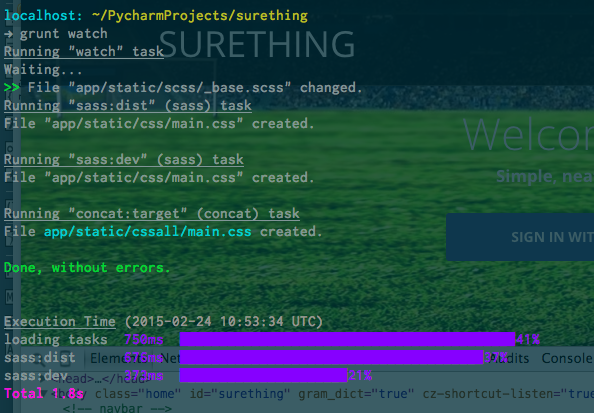
\includegraphics[width=.60\textwidth]{impl/images/gruntInAction}
		\caption{A screenshot from the terminal output running Grunt.} \label{fig:using:gruntinaction}
	\end{center}
\end{figure}
	
In addition, RequireJS  \citep{documentation:RequireJS}, a powerful asynchronous script loader will be used for effective management of JavaScript dependencies. It can load modules in asynchronous manner if desired and thus improve overall website performance.

\subsection{Back End}
\label{subsec:backend}
For making an accurate prediction the application requires latest football data. Live data would have to be frequently loaded into the system and processed in an appropriate way. Therefore, there would be a need for at least one separate module dealing with a third party football data API and containing business logic to manipulate the received data. The API wrapper is expected to be integrated into the web application, but separated from the presentation, it also has to be relatively easy to execute as a standalone module, encouraging a nicely decoupled design. 

Based on the above assumptions, Python was chosen as the primary back end language. The language is known for being well suited for data manipulation and analysis, and is therefore used in scientific computing and other highly quantitative domains, for example physics and finance. First of all, Python is a very effective language to be used for data processing. When processing a large amount of data, memory use management becomes very important. Python provides optimised syntax for processing a sequence, such as generator expressions. Generators enable iteration over a sequence without placing a new list, set, or dictionary into the system memory \citep{book:Phillips2010Python3ObjectOrientedProgramming}. Secondly, it is known for being easy to learn and use. This will hopefully allow to increase the speed of development, leaving plenty of time for identifying the bottlenecks and optimising the code. 

The back end of the web application will be built using Python web framework Flask \citep{documentation:Flask}. It is a lightweight framework (the official name is "Python microframework") with a great choice of third-party libraries (e.g. Flask-SQLAlchemy or Flask-Login) that can extend the feature set of the framework core in various ways. Flask application is minimalist to begin with, but it can grow with the project needs. For the purpose of this project this is an advantage compared to the full-featured frameworks like Django that have a lot of functionality already built-in in the basic installation. In addition, availability of developer-friendly documentation and low learning curve makes Flask a short way to get a simple, Python-powered web site up and running. Therefore, Flask appears to be a great choice for a small project like SureThing. 

SQLAlchemy was chosen as database solution for this project \citep{documentation:SqlAlchemy}. This is a powerful database framework that supports several databases back ends and offers the high-level Object Relational Mapper (for short, ORM). Using ORM provides a great level of abstraction when working with databases. For example, SQLAlchemy uses classes that map to each table in a database. This means that the records interaction can be kept the same regardless of the underlying database system. This offers a lot of flexibility and, for example, allows to use different database systems for development and production environment. According to \citet{book:Grindberg2014FlaskWebDevelopment}, "Flask-Migrate extension, based on a migration framework Alembic and written by a lead developer of SQLAlchemy, provides a powerful solution to handle database alterations and make database schema updates easily manageable" 

\section{Application Architecture}
\label{sec:applicationarchitecture}
Application architecture is a base of a good quality software. The architecture of SureThing was from a big part dictated by the used framework Flask, that uses a variation of MVC for Python called "MTV" (Model-Template-Controller). \citet{article:goodArchitecture} in his blog post describes this pattern in the following way:

\begin{quote}
"The template contains HTML content and presentation logic. It is written in a templating language ... It gets data from the view and outputs a web page. The view (also sometimes called “controller”), written in Python, is just glue code. It uses the web framework to put everything together. The model layer is essentially a persistence layer: its most important dependency is SQLAlchemy. The model knows how to save the data, constituting the most reusable code in the entire project."
\end{quote}

However, on the top of the standard MVC architecture SureThing requires few extra components to manage the loading of the data from an external source. Hence, this is the final layout of the application architecture:

\begin{itemize}
    \item \textbf{Model Layer.} Contains Python classes that represent database models and related logic. According to \citet{article:goodArchitecture}, model layer "represents the essence of [the] system without the details of a user interface."
    \item \textbf{View Layer.} Holds association between URL rules and view functions that are defined with a help of a module-level decorator \emph{route()}. Below can be found an excerpt from the application code, a header of a view function that represents the dashboard page. When a browser requests \url{/dashboard} URL, the associated view function is called and the return value is sent back to the browser. 

\begin{figure}[H]
    \begin{center}
        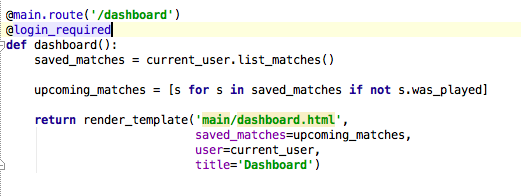
\includegraphics[width=.70\textwidth]{impl/images/routeExample}
        \caption{Dashboard view function.} \label{fig:using:routeexample}
    \end{center}
\end{figure}     
        
    \item \textbf{Template Layer.} This is the mediator layer between an HTTP request and the application logic. It consists of a number of Jinja2 templates holding only     presentation logic. 
    \item \textbf{External Services Layer} \citep{article:goodArchitecture}. Contains API wrapper class that accesses and manipulates live football data. In general, the functionality of the application can be further extended in many ways. In the future, Football-API might not be the only external source of data. The project might make use of another third-party API or even use web scraping technique to extract data from other websites . Eventually, all additional modules related to the interaction with external sources of data will become part of this layer.
    \item \textbf{Threading.} The application requests live football data frequently. Loading the data is a costly I/O operation that may become a bottleneck unless performed asynchronously. Threading component of the apllication defines a class \emph{DataUpdateThread} that takes care of writing the data to the server every 100 seconds. This task is performed in a separate thread. 
\end{itemize}

During the development process, a lot of effort was put into keeping the Template Layer as thin as possible in order to reduce the loading time in the browser and improve the overall performance of the application.

\section{Patterns And Conventions}
\label{sec:patternsandconventions}
Flask offers an excellent extendable core of functionality; its API is also very minimalistic and easy to understand. One of the  main advantages of this framework is that it gives developer a lot of freedom to decide how to structure the application. As \citet{article:howIstructureMyFlaskApps} puts it: " without patterns or conventions your applications will loose architectural integrity and be difficult to understand by others". In this section a number of various patterns, conventions and tools used during the implementation phase will be described and explained. 

\subsection{Application Factory}
\label{subsec:applicationfactory}
The use of factory pattern is crucial to a Flask application. For example, SureThing app defines various configurations to be used in different environments (development, testing, production). However, because the application instance is created in the global scope, there is no way to apply those configurations. The problem is that "by the time the script is running, the application instance has already been created, so it is already too late to make configuration changes" \citep{book:Grindberg2014FlaskWebDevelopment}. To get around this problem a creation of the application was moved into a separate function, \emph{create\_app()}. The name of configuration name is passed into the function as a parameter. This solution also allows us to create multiple instances of the application and make testing of various confurations easier \citep{documentation:FlaskApplicationFactories}.

\begin{figure}[H]
	\begin{center}
		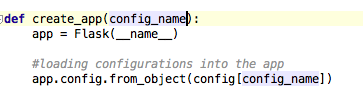
\includegraphics[width=.50\textwidth]{impl/images/createApp}
		\caption{Function responsible for creating the application instance.} \label{fig:using:createapp}
	\end{center}
\end{figure}

\subsection{Blueprints}
\label{subsec:blueprints}
Blueprints are related to the View Layer introduced in the section Application Architecture \ref{sec:applicationarchitecture}. A large application is divided into smaller parts and each part is implemented with help of a blueprint. This concept helps to develop a \emph{modular} web application. SureThing was divided into two parts: \emph{main} and \emph{auth}. \emph{auth} holds the endpoints associated with the authentication and user profile related tasks, for example \emph{login()}, \emph{edit\_profile()}. On the other hand \emph{main} is in charge of the rest of the application. Notice how those different blueprints are registered on the application instance inside the \emph{create\_app()} function:

\begin{figure}[H]
	\begin{center}
		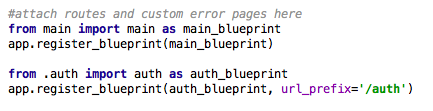
\includegraphics[width=.50\textwidth]{impl/images/blueprintsRegistration}
		\caption{Blueprints registration.} \label{fig:using:blueprintsregistration}
	\end{center}
\end{figure}

\subsection{Database Migrations}
\label{subsec:databasemigrations}
The database scheme for this project was designed in an iterative way, models and relationships between them were added gradually as the application was growing. Therefore, it was crucial to find a tool that allows effortless updates of the database. To manage frequent database updates was used Alembic database migration tool that was developed specifically by Mike Bayer, the author of SQLAlchemy. The tool can be added to Flask as an external plugin, Flask-migrate. After installation and initial configuration of the plugin, it allows to migrate the database with two simple commands to be subsequentially run in the terminal: \emph{db upgrade} and \emph{db migrate}. Alembic makes migration easier and prevents the developer from the necessity to delete and recreate the database each time there is a need for migration.

\subsection{Exceptions}
\label{subsec:exceptions}
In general, it is considered a good practice to take advantage of standard libararies of a programming language, in our case Python. First of all, it allows developer to save time implementing a piece of functionality from scratch. Secondly, it makes it easier for other developers to read and maintain the code. Exceptions are built into Python at the language level. Using them will lead to cleaner code and will not have any impact on the performance. "In a way, try blocks are like transactions. [The] catch has to leave ... program in a consistent state, no matter what happens in the try. For this reason it is good practice to start with a try- catch- finally statement when you are writing code that could throw exceptions " \citet{book:martin2011robert}.
 
SureThing will make use of Exceptions in order to identify and manage failures when making an API call over HTTP. The FootballAPIWrapper class has a private method that calls the API and collects the data in a JSON format from the remote server: \emph{\_call\_api(action=None, **kwargs)}. The method takes into account the possibility of errors occuring during code execution. When the program calls the API, either JSON data is returned or an Exception is thrown. 

As it can be seen from the method definition above, one of the required parameters is \emph{action} that is set to None, unless the value is passed in during the method call. Action is a string that needs to be added to the base url in order to indicate the set of data that is being accessed. Specifying the action is required by the API and the possible values of the parameters (actions) are: competition, standings, today, fixtures, commentaries. For example action \emph{today} will returns the matches scheduled today. The \emph{\_all\_api} method will raise an Exception, if the action is not being supplied. Various exceptions are thrown when the program is attempting to connect to the remote server \citep{article:httpRequestsExceptions}. Python library \emph{requests} is used to take care of this type of errors \citep{documentation:PythonRequests}. If the domain name does not resolve, the HTTP request will fail before we establish connection. In that case, the program will throw a \emph{requests.exceptions.ConnectionError}. If the remote server is not functioning or the request is structured incorrectly, the server will respond with an bad response status code and the \emph{\_call\_api} method will raise a \emph{requests.exceptions.HTTPError}.

\section{Other Implementation Processes}
\label{sec:otherprocesses}
In this section a number of other implementation processes and used tools will be discussed.

\subsection{PEP8}
\subsection{PyLint}

\subsection{Version Control}
\label{subsec:git}
Git version control system was used throughout the development process. Git is known for being a very useful tool for collaboration across teams of developers. However, it has also many benefits for a solo developer. For example, it helps to track changes and restore previous versions of a project, as well as view the code at any point in the past. The project codebase was uploaded to GitHub that is "a web-based Git repository hosting service, which offers all of the distributed revision control and source code management (SCM) functionality of Git as well as adding its own features... [It also] provides web-based graphical interface" \citep{wiki:GitHub}. For this project GitHub issue tracker was used as a "to-do list" to keep the record of tasks ("issues" in GitHub terminology) that needed to be completed in each agile iteration. Custom labels were used to distinguish different types of issues in the GitHub issue tracker, for example, "performance", "design", "bug", "optional", etc. 

\begin{figure}[H]
	\begin{center}
		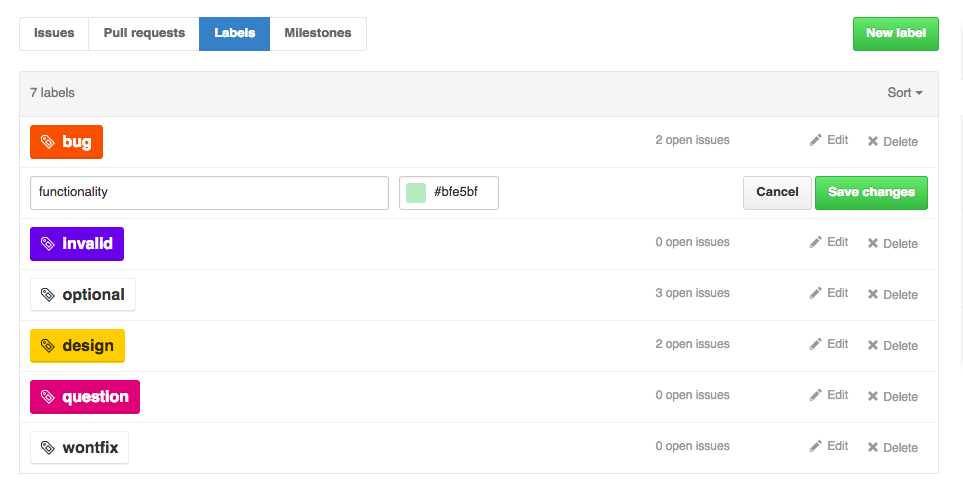
\includegraphics[width=.90\textwidth]{impl/images/githubLabelsChoice}
		\caption{GitHub allows developers to add custom labels.} \label{fig:using:githublabelschoice}
	\end{center}
\end{figure}

GitHub also allows the users to filter out the issues of a similar type, based on the assigned label.

\begin{figure}[H]
	\begin{center}
		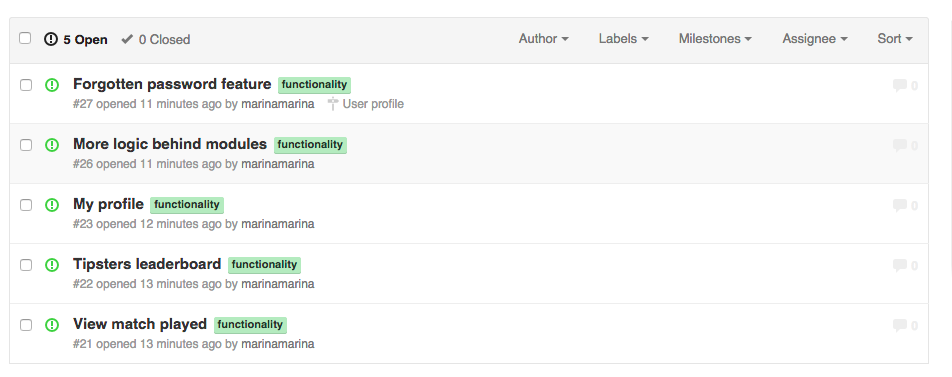
\includegraphics[width=.90\textwidth]{impl/images/githubFunctionalityIssues}
		\caption{GitHub. Issues related to the functionality of the application.} \label{fig:using:githubfunctionalityissues}
	\end{center}
\end{figure}

Critically speaking, I missed the option to assign issues various level of importance and order the issues based on their priority.

\subsection{Own Validation in Forms}
\label{subsec:validations}
Flask-WTF is a Flask extension that offers integration with WTForms and it was used to handle forms in this project. In order to make sure the application is secure, the validation has to be implemented preferably on the server side or both on the client- and server-side of the application. WTForms has many built-in validators that can simplify developer's life. For example \textbf{DataRequired} makes the input field mandatory, \textbf{Email} checks that the provided input is a valid email address, \textbf{EqualTo} helps to ensure that the passwords in the fields "Password" and "Confirm Password" supplied during the user registration are identical. However, sometimes the built-in functionality does not cover all the application needs. In that case, there is an option to create a custom validator that is a basically a Python function returning another function (a validator) that throws an exception every time the user violates the prescribed validation rule. Custom validators can be imported into the module describing forms and used in the same way as a built-in validator would be used. I have separated the validators out into a separate module. The set of custom validators can be further extended, however, there is just one at the moment: \emph{validator\_user\_already\_registered()}. 

\begin{figure}[H]
	\begin{center}
		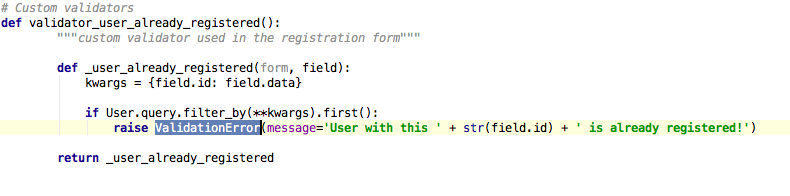
\includegraphics[width=.90\textwidth]{impl/images/customValidator}
		\caption{Validator function that checks if user with this username has already been registered with the SureThing application} \label{fig:using:customValidator}
	\end{center}
\end{figure}

In the example above the validator function checks if a user with provided username is already in the database. If the user is found, the ValidationError exception is thrown and the new user is prevented from submitting the form.

\subsection{Custom Macros}
Jinja2 is a default template engine that comes in one package with Flask. It is also one of the most widely used template engines for Python. In order to add some extra presentation logic to our application, custom macros can be used. Jinja2 macro is simply a template function that can be used within HTML in order to avoid developers writing repetitive code. For this project I found macros extremely useful. Custom macros were separated out into a separate template file \emph{\_macros.html}.

One of the example usages was rendering form fields. Each form field related macro contained a piece of HTML code specifically designed for forms in this application, as well as logic for dispaying error messages. Among this type of macros can be named \emph{render\_field(field)}, \emph{render\_checkbox(field)}, \emph{render\_submit\_field(field)}. Some of those macros needed to be adjusted to enable their usage in a specific view. These are the examples of such "adjusted" macros: \emph{render\_submit\_field\_match\_preview(field)}, \emph{render\_embedded\_field(field)}. For example, \emph{render\_field} takes care of rendering any standard input field accross the application, whereas \emph{render\_embedded\_field(field)} manages rendering an input field embedded within a prediction module on the Upcoming Match View. 

Another macro, \emph{teamkitimage(match, home=1)} renders an image representing a football club. Based on the provided arguments, the function displays an image of a home or away team kit for a specific club. 

\subsection{Integration with third-party API}
Many production Python web applications rely on external application programming interfaces (APIs). API can be also reffered to as "third party services" or "external platform" \citep{article:API_Integration}.  SureThing requires constant access to current football data. After choosing an appropriate API, it has to be integrated into the application. 

There is a variety of tools available for developers for accessing web APIs. Those three options were considered when choosing an appropriate tool:
	
\begin{itemize}
	\item Helper library (such as Runscope or Apiary)
	Using a helper library has an overhead of learning how to use another piece of software.
	\item urllib2, standard Python module
	\emph{urllib2} module offers very simple implementation and provides most of the required HTTP capabilities, but the API is thoroughly broken and features critical for performance are missing, for example connection re-using/pooling. 
	\item urllib3
	\item requests, another Python library for handling HTTP requests. It offers a lot of control over the HTTP calls through the use of its powerful features.
\end{itemize}
		
After some experiments with other urllib2, urllib3 and requests, \emph{requests} was chosen as the libarary for this project.
		
All interaction with the Football-API, including processing the received data, was separated out into a module \emph{football\_api\_wrapper.py} or just "wrapper" for short. This module contains only one class, FootballAPIWrapper. Fields of the class accomodate the key elements of the interaction with the API that will be re-used in different methods of the wrapper, for example base url, path to the data directory.
	
\begin{figure}[H]
	\begin{center}
		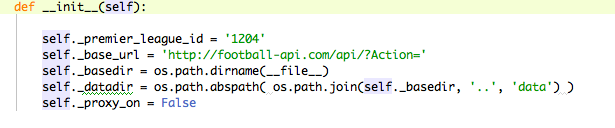
\includegraphics[width=.90\textwidth]{impl/images/footballApiWrapperFields}
		\caption{Football API wrapper, fields} \label{fig:using:footballapiwrapperfields}
	\end{center}
\end{figure}
	
To get the response from Football-API takes about 11s, therefore it is nessessary to move the API calls into a task queue so they do not block the HTTP request-response cycle for the rest of the web application.

\subsection{Visual Effects}
A number of visual effects was implemented with the help of jQuery, AJAX and the Websockets (Flask extention Flask-SocketsIO) to improve the user experience. 

\subsubsection*{Alerts}
A good example is an alert dismissal. SureThing generates many alerts that give the user feedback with regards to the action they have just taken. User has to dismiss the alert manually each time. To avoid this extra thing for a user to do, the alerts are removed from the page using jQuery fadeOut() and then slideUp() animation methods that fades the pop-up and then removes it with a sliding motion after 200ms of its appearance on the page. For compactness the screenshot shows the page opened in a browser simulation of an iPhone screen size. Responsive web design with regards to this project will be examined in more detail in the following subsection.

\begin{figure}[H]
	\begin{center}
		
\includegraphics[width=.60\textwidth]{impl/images/alert}
		\caption{An example of an alert on the page appearing after user has logged out} \label{fig:alert}
	\end{center}
\end{figure}

\begin{figure}[H]
	\begin{center}
		
\includegraphics[width=.60\textwidth]{impl/images/alertFadeOut}
		\caption{The same alert fading out.} \label{fig:alertFadeOut}
	\end{center}
\end{figure}

\subsubsection*{New message notifications}
Another example is a new message notification. Once user received a new in-app message notifying them about the results of their bets, the envelope-shaped icon on the top navigation menu that represents the in-app Inbox turns orange. 

\begin{figure}[H]
	\begin{center}
		
\includegraphics[width=.60\textwidth]{impl/images/alertFadeOut}
		\caption{The same alert fading out.} \label{fig:alertFadeOut}
	\end{center}
\end{figure}

When user navigates to the Inbox and reads or deletes all the new messages, the icon immediately turns greyindicating that there are no more unread messages in the box.
 
\begin{figure}[H]
	\begin{center}
		
\includegraphics[width=.60\textwidth]{impl/images/newMessagesDesktopView}
		\caption{You have new messages. Desktop View.} \label{fig:newmessagesdesktopview}
	\end{center}
\end{figure}

This is what the same top navigation menu looks like for mobile users. 

\begin{figure}[H]
	\begin{center}
		
\includegraphics[width=.60\textwidth]{impl/images/newMessagesMobileView}
		\caption{You have new messages. Mobile View.} \label{fig:newmessagesmobileview}
	\end{center}
\end{figure}

User has opened the last unread message and the message icon has turned grey. Notice, how the top navigation menu partly covers the message view. The menu rolls back into a compact mode once the user clicks on the menu icon in the top right corner.

\begin{figure}[H]
	\begin{center}
		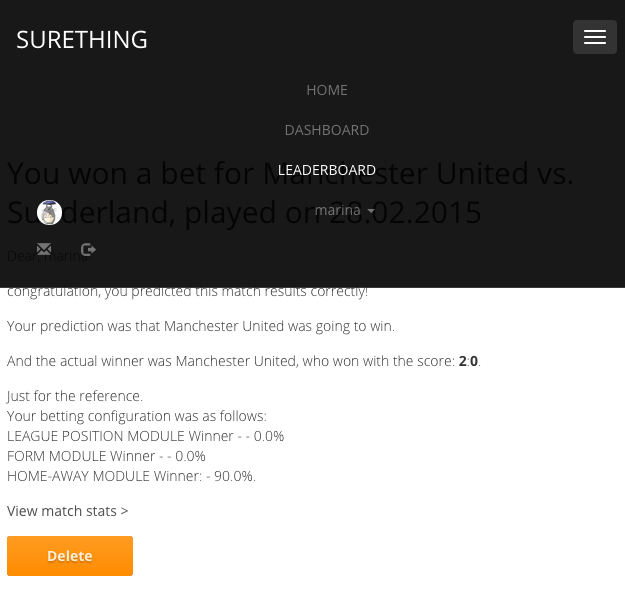
\includegraphics[width=.60\textwidth]{impl/images/noMoreNewMessages}
		\caption{User just read the last new message, the icon turns grey.} \label{fig:nomorenewmessages}
	\end{center}
\end{figure}

\subsection{Responsive Design}
According to the popular portal Statista, "As of 2013, worldwide mobile phone internet user penetration was 73.4 percent. In 2017, figures suggest that more than 90 percent of internet users will access online content through their phones" \citep{statistaReport}. There is no doubt that developers need to adapt to the increasing combinations of screen resolution and browsers used by people to access information online. The solution to the expanding variability of the web is to develop a layout that can adapt to any viewport. This approach is known as \emph{responsive web design}. The term was first used by Ethan Marcotte. He combined three already known techniques (flexible grid layout, flexible images, and media and media queries) into a unified approach \citep{book:frain2012responsive}. 

Based on the above, we should assume that the majority of users will access our website through a device that is not a desktop. We need a good fluid grid to build a responsive web application. To handle the responsiveness and to increase development speed SureThing utilises Bootstrap framework \citet{documentation:Bootstrap3}. that offers an responsive fluid grid system that can adjust to the variety of devices or screen sizes. The framework has also predefined classes that can be used to change the page layout options, for example to specify how many columns in the grid system an element will occupy or to set the breakpoints at which the columns stacked on small devices will become horizontal on medium/large devices. 

SureThing is a fully responsive web application, and the minimum screen resolution supported is 640 x 960 pixels (an example device is an iPhone 4). These are the screenshots of some of the application pages tested with this resolution:

\begin{figure}[H]
	\begin{center}
		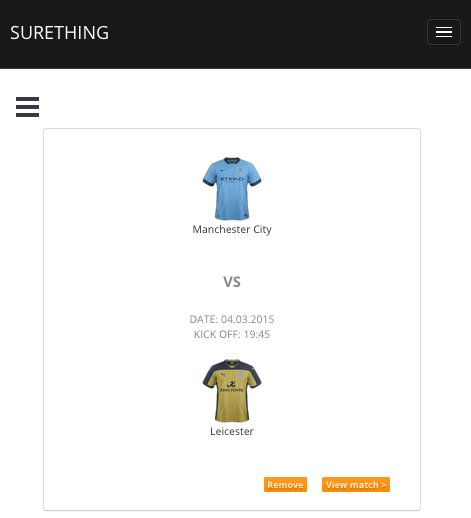
\includegraphics[width=.50\textwidth]{impl/images/responsiveDashboard}
		\caption{Dashboard view, DVGA screen size.} \label{fig:using:responsivedashboard}
	\end{center}
\end{figure}

\begin{figure}[H]
	\begin{center}
		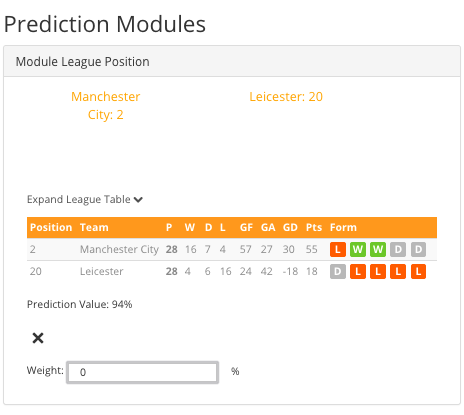
\includegraphics[width=.50\textwidth]{impl/images/responsiveModuleLeaguePosition}
		\caption{Module League Position in the Upcoming Match View, DVGA screen size.} \label{fig:using:responsivemoduleleagueposition}
	\end{center}
\end{figure}

\section{Features Implementation}
In this section will be described the technical details of the project implementation. Each susbsection is bound to the high level feature of the application, as indroduced in the chapter "Requirements Analysis" \ref{sec:functionalrequirements}. "User journey", or possible user interactions with the system, will be demonstrated for each view.

\subsection{Authentication and User Profile}

\subsubsection*{Authentication}
The application requires authentication functionality. In order to simplify the development process, a useful Flask extention, Flask-Login, was utilised to handle the common tasks of logging in and out, as well as new users registration. For the new users application offers a registration form. On form submission, SureThing sends user an email with verification token, expecting them to confirm the email address and complete the registration. It should be noted that both username and email address provided during the registration should be unique, otherwise the application throws a validation error. The screenshot below is an example of what happens when a new user tries to register using an email address that is already in the database:

\begin{figure}[H]
	\begin{center}
		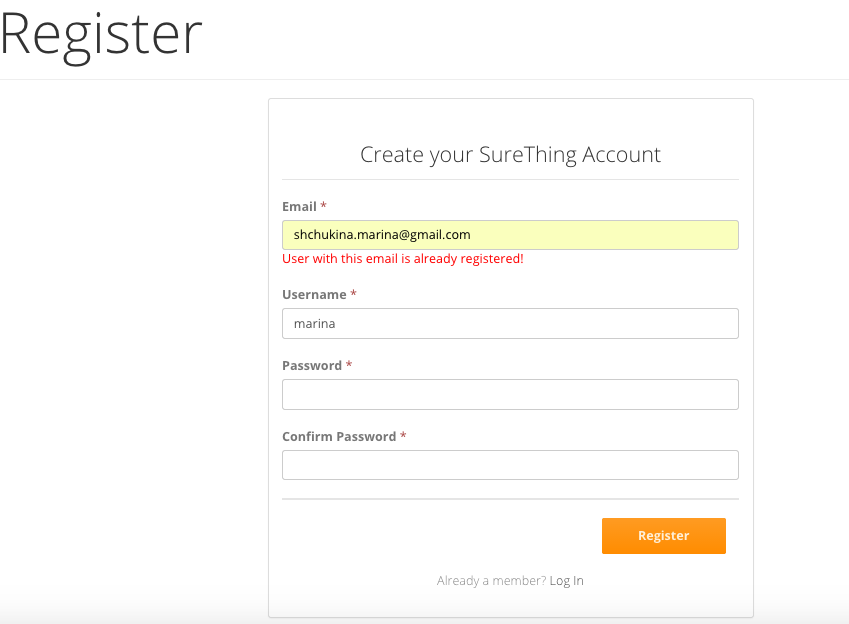
\includegraphics[width=.90\textwidth]{impl/images/registrationFormError}
		\caption{SureThing offers registration form for the new users. However, the email address is expected to be unique.} \label{fig:registrationformerror}
	\end{center}
\end{figure}

Once a user has created a SureThing account, they can login using a standard login form.  An email address and a password are both required fields. A validation error will be thrown in case the provided email or password are invalid, or the user with the provided email address was not found in the database.

\emph{Gravatar} is an abbreviation for "Globally recognized avatar" and it is one of the most popular avatar services. User can register with the service (\url{http://gravatar.com}) and upload an image that can be used as avatars across many popular websites, such as GitHub (\url{http://www.github.com}), Stackoverflow (\url{http://www.stackoverflow.com}) and WorldPress (\url{http://www.worldpress.com}). Gravatars are integrated into the SureThing, and a newly registered user does not have to upload an avatar image to be used in our application. The app will access the avatar associated with user's email address and pull it from the Gravatar servers. An authorised user will see the icon with their avatar picture in the top right corner of the application navigation menu, as it can be seen in the screenshot below:

\begin{figure}[H]
	\begin{center}
		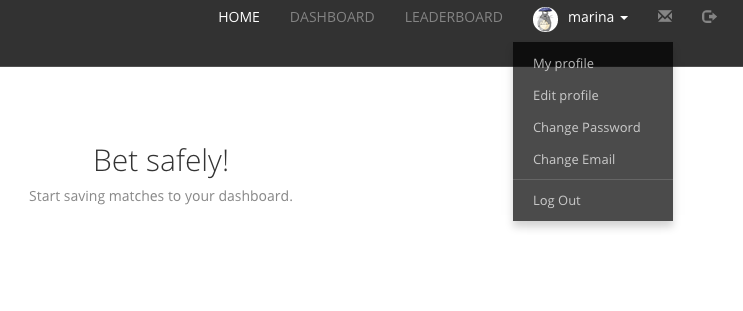
\includegraphics[width=.90\textwidth]{impl/images/gravatar}
		\caption{User settings and the profile page can be accessed by clicking on the avatar icon located on the application navigation menu panel.} \label{fig:gravatar}
	\end{center}
\end{figure}

In case the user is not registered with the Gravatar, SureThing will generate a dummy avatar to be used in the application.

\begin{figure}[H]
	\begin{center}
		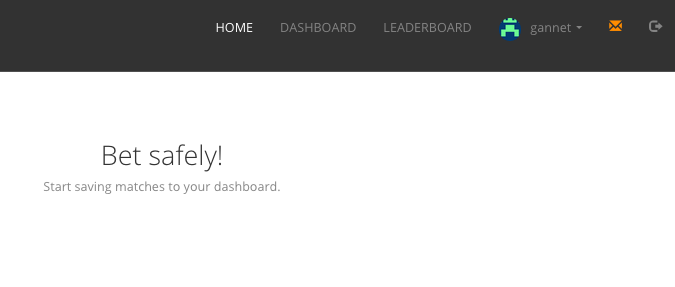
\includegraphics[width=.90\textwidth]{impl/images/dummyGravatar}
		\caption{An example of a dummy gravatar for user \textbf{gannet}, who is not registered with Gravatar services.} \label{fig:dummygravatar}
	\end{center}
\end{figure}

\subsubsection*{User Profile}
The options available in the dropdown menu, as displayed in the figure ~\ref{fig:gravatar}, enable the users editing their profiles, changing password and email address. 

\begin{figure}[H]
	\begin{center}
		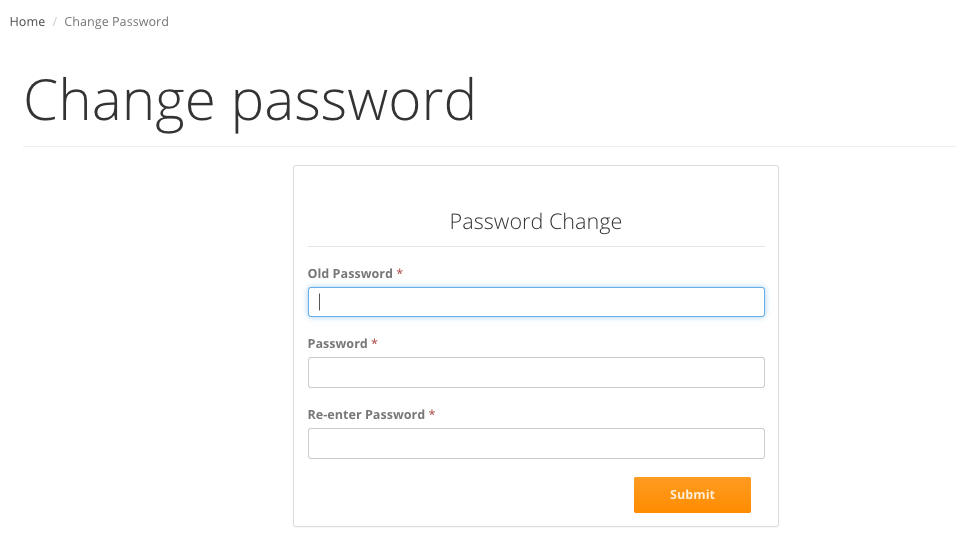
\includegraphics[width=.90\textwidth]{impl/images/changePassword}
		\caption{Users can change their passwords for security reasons.} \label{fig:changePassword}
	\end{center}
\end{figure}

\begin{figure}[H]
	\begin{center}
		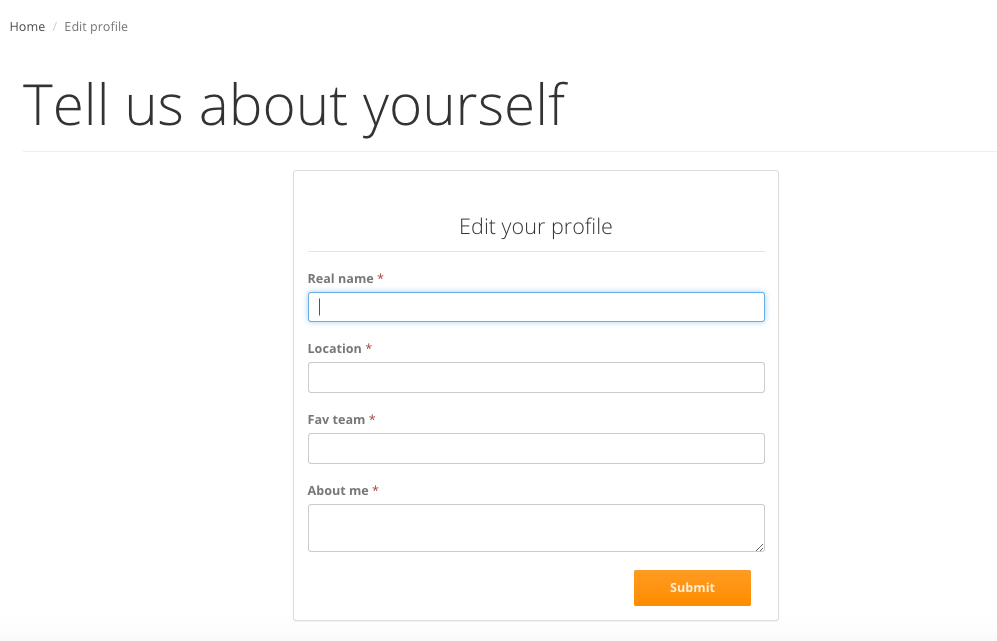
\includegraphics[width=.90\textwidth]{impl/images/editProfile}
		\caption{After the registration users can share more information about themselves by editing their profile.} \label{fig:editprofile}
	\end{center}
\end{figure}

Clicking on the dropdown option "Profile" will take the user to a separate page containing all the information about the user, for example: profile information, preferences, section "about me", recent won bets including the prediction weights used for those bets, etc. 

\begin{figure}[H]
	\begin{center}
		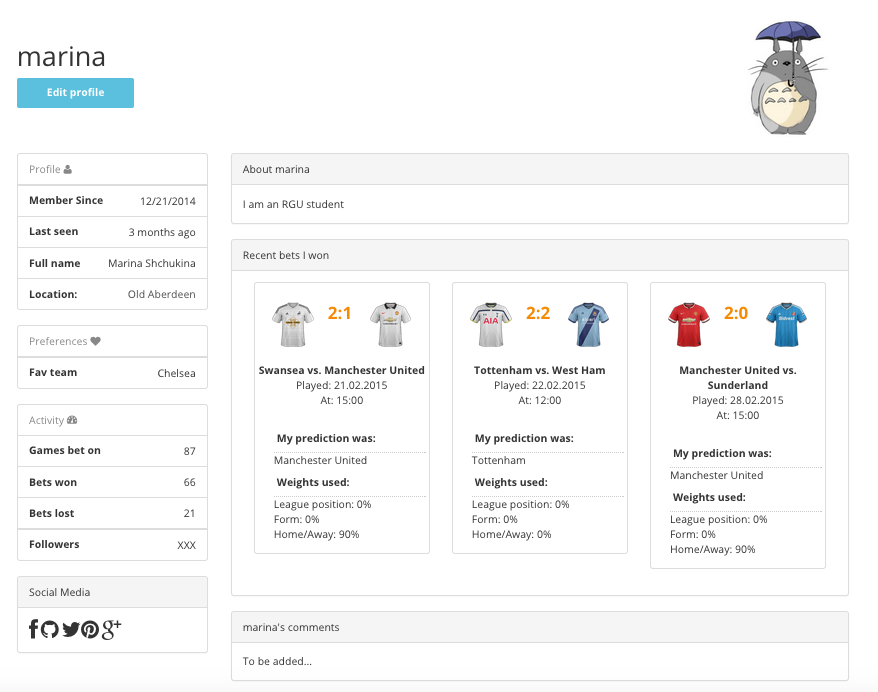
\includegraphics[width=.90\textwidth]{impl/images/profile}
		\caption{User profile page.} 
		\label{fig:profile}
	\end{center}
\end{figure}

\subsubsection*{User Journey}
\label{subsec:authandprofileuserjourney}
From the User Profile page user can navigate to the "Edit Profile" form by clicking on the light blue "Edit Profile" button located in the top left corner of the profile page. 

\subsection{Matches Overview}
Matches Overview is a view displayed on the main page of the application. It contains lists of upcoming and played matches and the user can toggle between those two lists using navigation buttons. In both lists matches are grouped by dates as follows:

\begin{figure}[H]
	\begin{center}
		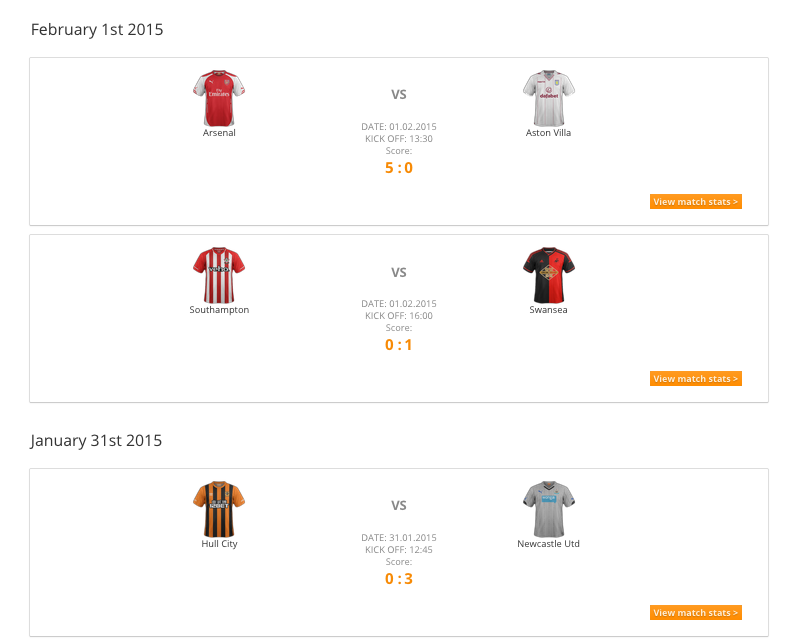
\includegraphics[width=.90\textwidth]{impl/images/matchesGrouped}
		\caption{Matches in the overview are grouped by dates sorted in ascending order.} \label{fig:using:matchesgrouped}
	\end{center}
\end{figure}
 
Each panel representing a match contains the most basic information about the event, such as names of participating teams, kick-off date and time. The screenshot below is an example of a panel displaying an unplayed match. The navigation buttons can be seen just above the first match in the list. Match already saved to the Dashboard by the authenticated user is indicated by a floppy disk icon on the right hand side of the panel.

\begin{figure}[H]
	\begin{center}
		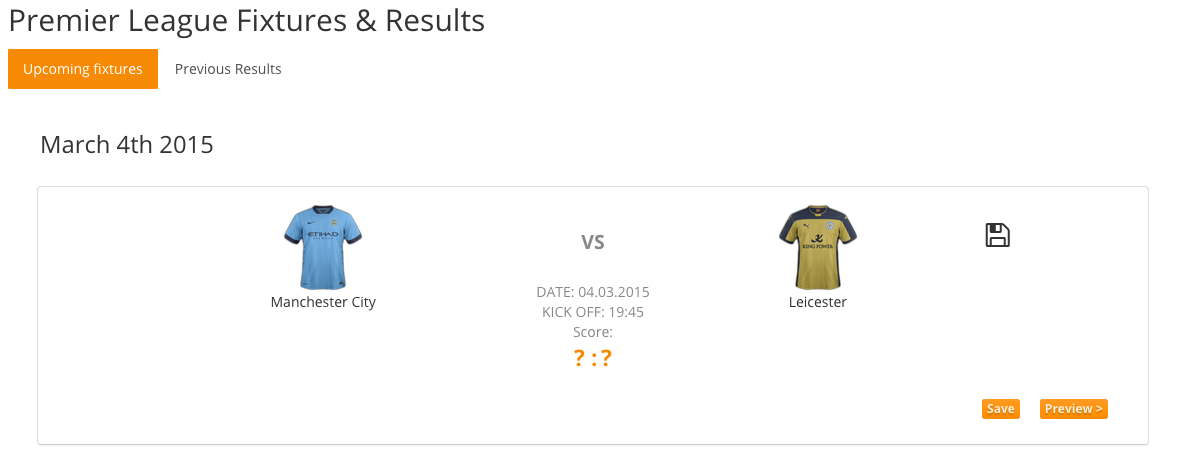
\includegraphics[width=.90\textwidth]{impl/images/unplayedMatch}
		\caption{Example of an unplayed match displayed in the overview.} \label{fig:using:unplayedmatch}
	\end{center}
\end{figure}

Below can be found a screenshot of a played match panel. Notice that the final score of the match is displayed and instead of two buttons "Save" and "Preview" there is only one button - "View match stats".

\begin{figure}[H]
	\begin{center}
		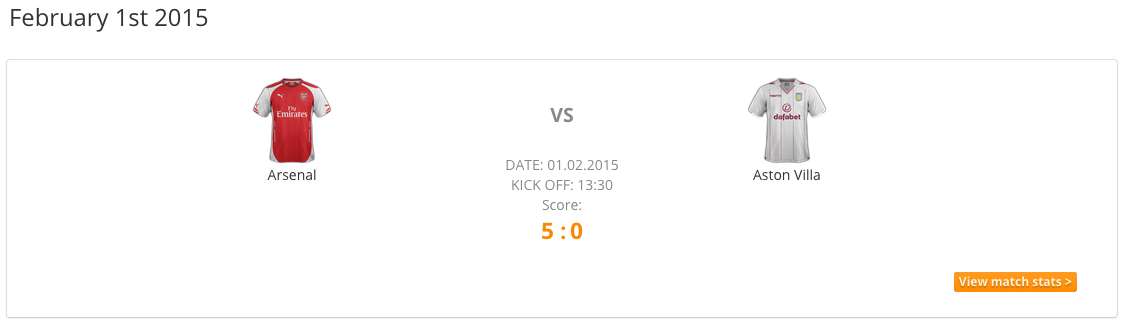
\includegraphics[width=.90\textwidth]{impl/images/playedMatch}
		\caption{Example of a played match displayed in the overview.} \label{fig:using:playedmatch}
	\end{center}
\end{figure}

In case the match is being played at the very moment, it still belongs to the list of "unplayed" matches and is displayed with a small badge "LIVE", indicating live event. A match is considered as "played" as soon as the full time score is available. Hence, it is possible to make "bets" until the moment the match is considered "played".

\begin{figure}[H]
	\begin{center}
		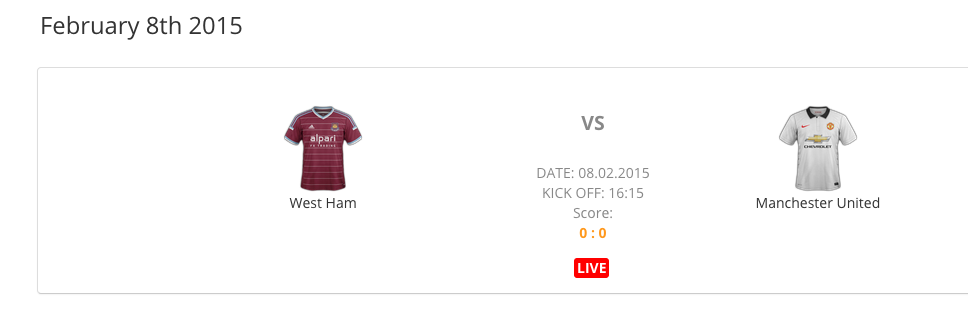
\includegraphics[width=.90\textwidth]{impl/images/liveMatch}
		\caption{Example of a live match displayed in the overview.} \label{fig:using:livematch}
	\end{center}
\end{figure}

\subsubsection*{User Journey}
\label{subsec:matchesoviewuserjourney}
Just above the list can be found simple navigation allowing to switch between the lists of unplayed and played matches. On the right hand side of each list item there is a "Preview" button for an upcoming match and a "View match stats" button for a played match. By clicking those buttons user can navigate to views with more detailed information about the match (\emph{Upcoming Match View} or \emph{Played Match View}). User can save the match to the dashboard by clicking "Save" button. This action can be carried out only for an unplayed match.  

\subsection{Upcoming Match View}
\label{subsec:implementupcomingmatchview}
Implementation of this view was one the most complex development tasks of the whole project. This is the essense of SureThing - view allowing the user to predict match results. 

Authenticated SureThing user can navigate to this view either by clicking a "Preview" button on an upcoming match panel in the \emph{Matches Overview} or by clicking the same button on a saved match panel in the user \emph{Dashboard} (if the match has already been saved by the user). Depending on the user route to this view, the Upcoming Match Preview will be displayed differently.

\subsubsection*{Read-only mode}
If the user is coming to the Upcoming Match Preview from the \emph{main page}, the view will display the match header (containing general information about the teams, last played game, match kick-off time and date, etc.) and a list of prediction modules with \textbf{prediction values} calculated based on the relevant piece of statistics for each of the teams. These are the prediction modules available in this view: 

\begin{enumerate}
	\item Module League Position
	\item Module Form
	\item Module Home/Away
\end{enumerate}

"Save" button can be found at the very bottom of the view.

\begin{figure}[H]
	\begin{center}
		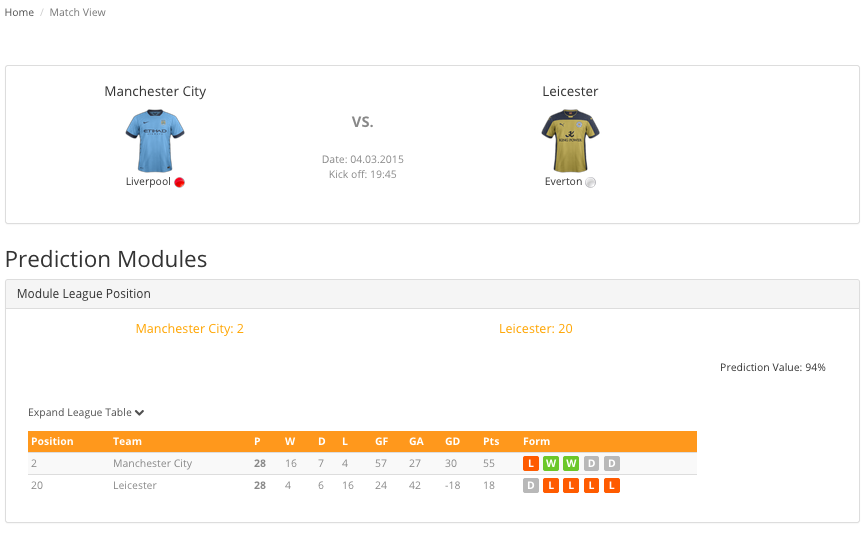
\includegraphics[width=.90\textwidth]{impl/images/upcomingMatchView}
		\caption{Upcoming Match View in the "read-only" mode: match header and the first prediction module, Module League Position.} 
		\label{fig:using:upcominmatchview}
	\end{center}
\end{figure}

This information should be sufficient for the user to decide, whether it is worth saving the match to the dashboard for a later revision. An unauthorised user would be able to see the same content, but the "Save" button will be disabled. We can say that if user navigates to the Upcoming Match View from the main page, they can see the view in the \textbf{read-only mode}. It is also important to note that this is one of few views that are available for an unauthorised user.

\subsubsection*{Prediction mode}
\label{subsubsec:predictionmode_implementation}
In case user has already saved the match to the dashboard and navigates to the Upcoming Match View by clicking on a saved match panel, the view will enable the prediction feature. This time the view is displayed in the \textbf{prediction mode}. In each of the prediction modules user will be able to see an embedded input field with weight percentages inside the field. Below can be found a screenshot of a same part of the view as the one above, displayed in prediction mode.

\begin{figure}[H]
	\begin{center}
		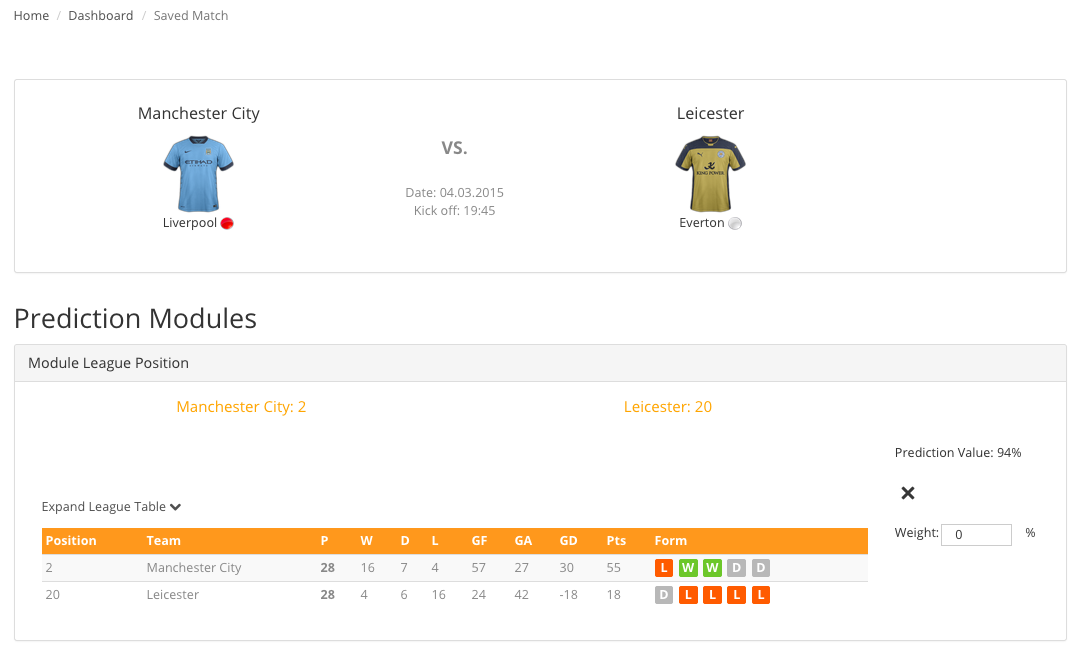
\includegraphics[width=.90\textwidth]{impl/images/upcomingMatchViewSM}
		\caption{Upcoming Match View in the "prediction" mode: match header and the first prediction module, Module League Position.} 	  \label{fig:using:upcominmatchviewSM}
	\end{center}
\end{figure}

The values displayed inside the fields will be used for calculating the overall match result prediction. If this is the first time user previews the match, the prediction weights will be either the \textbf{system default} (in case user has not set the prediction settings in the dashboard yet) or the \textbf{user default} prediction settings. If user has already visited this page before and set the match specific settings, the values displayed inside the input fields will be the \textbf{match specific} ones. Any module can be eliminated from the prediction by setting its weight to 0\%. The total sum of prediction weights must equal to 100\%.

These are the prediction modules available to the user in the prediction mode:

\begin{enumerate}
	\item Module League Position
	\item Module Form
	\item Module Home/Away
	\item User Hunch
\end{enumerate}

Notice, the extra module is available in this view - User Hunch. This module is very important to the prediction process. User can personalise the prediction by choosing Home, Away or Draw value in the User Hunch module panel. The module will be explained in more detail in the following subsection, "Prediction" \ref{subsec:prediction_implementation}

\begin{figure}[H]
	\begin{center}
		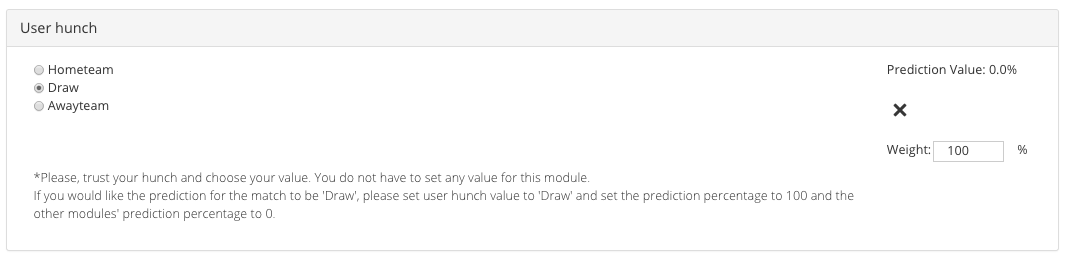
\includegraphics[width=.90\textwidth]{impl/images/userHunch}
		\caption{Module User Hunch.} \label{fig:using:userHunch}
	\end{center}
\end{figure}

The overall prediction is displayed underneath all modules, in a separate panel.

\begin{figure}[H]
	\begin{center}
		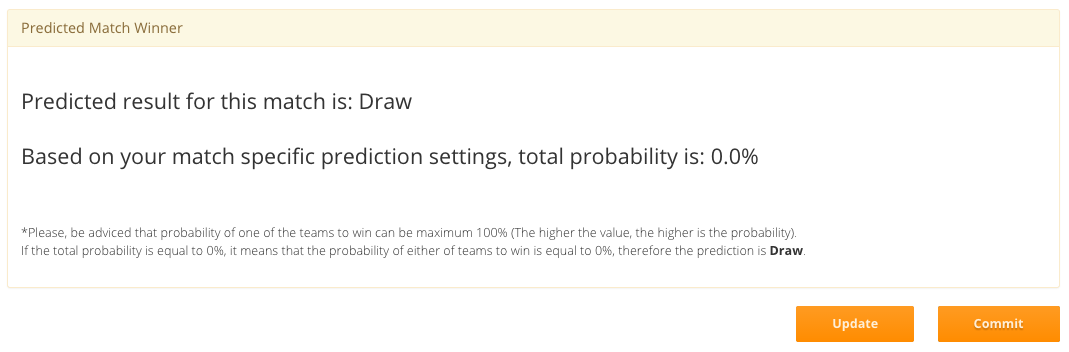
\includegraphics[width=.90\textwidth]{impl/images/prediction}
		\caption{Match result prediction.} \label{fig:using:prediction}
	\end{center}
\end{figure}

\subsubsection*{User journey}
\label{subsec:upcomingmatchviewuserjourney}
In the \textbf{read-only} mode the user can save the match to the dashboard by clicking "Save" button. 

In the \textbf{prediction} mode the user can update the prediction settings by overriding the current values in each of the input fields and pressing the button "Update" that is located at the bottom of the view. The overall prediction output will change every time the user updates the prediction settings or changes the hunch value. Once satisfied with the prediction outcome, the user can commit the match by pressing "Commit" button that is located next to "Update". Before the end of the match, the user can still navigate to the committed match view and see the all the details, including the prediction values, used weights and the final prediction. However, this time "Update" and "Commit" buttons will be disabled.

\begin{figure}[H]
	\begin{center}
		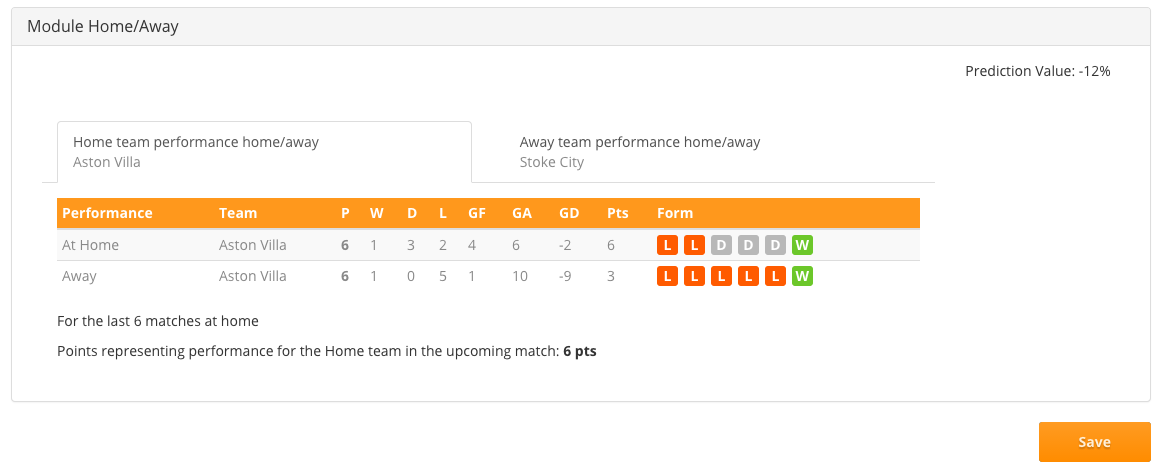
\includegraphics[width=.90\textwidth]{impl/images/matchoverviewex_from_main_page}
		\caption{An example of a prediction module in the Match Preview, user navigated from the main page.} \label{fig:using: matchoverviewex_from_main_page}
	\end{center}
\end{figure}

If the user comes to the upcoming match preview from the \emph{dashboard}, they will be able to see more information related to the actual result prediction and betting.
First of all, in each prediction module they will see an input fields for setting match specific prediction weights. Secondly, they will see a user hunch module. Finally, at the very bottom of the overview they will see calculated prediction result and two buttons - one to save the match specific settings and another to commit the bet.


most Explain how was implemented user hunch: combination of Flask Ajax and Sockets IO!!!
 
\subsection{Prediction}
\label{subsec:prediction_implementation}
After getting familiar with the \emph{Upcoming Match View}, the next logical step is to introduce the reader of this report to the Prediction feature of the application. This will aid understanding how to use the \emph{Upcoming Match View} and what kind of information this view offers to an intended user. The implementation of the Prediction feature was already briefly outlined in the chapter "Requirements Analysis", subsection "Prediction" \ref{subsec:prediction_requirements}. In this part of the report, I would like to illustrate the practical side of this feature. In this subsection will be explained several levels of prediction settings used in the application, the way the prediction values are calculated and the logic behind the prediction of the match result. 

\subsubsection*{Three levels of prediction weights}
SureThing has three levels of prediction settings or weights. Firstly, the \emph{system default} prediction settings - a set of weights "recommended" to the new users by the system. Once the user is registered with the application, they can set their own set of weights that will override the system default settings - \emph{user default} prediction settings. This can be done through a "Prediction Settings" form, as explained in the subsection "Dashboard" \ref{subsec:dashboard}. From the moment those weights are saved in the database, they will apply to every newly saved match. The application also enables setting \emph {match specific} prediction settings that will only apply to one match. User can set match specific weights through the Upcoming Match view page in prediction mode \ref{subsubsec:predictionmode_implementation}.

The prediction of match result is expressed in percentage and is calculated as a weighted average of a set of prediction values with different levels of relevance. 

\begin{figure}[H]
	\begin{center}
		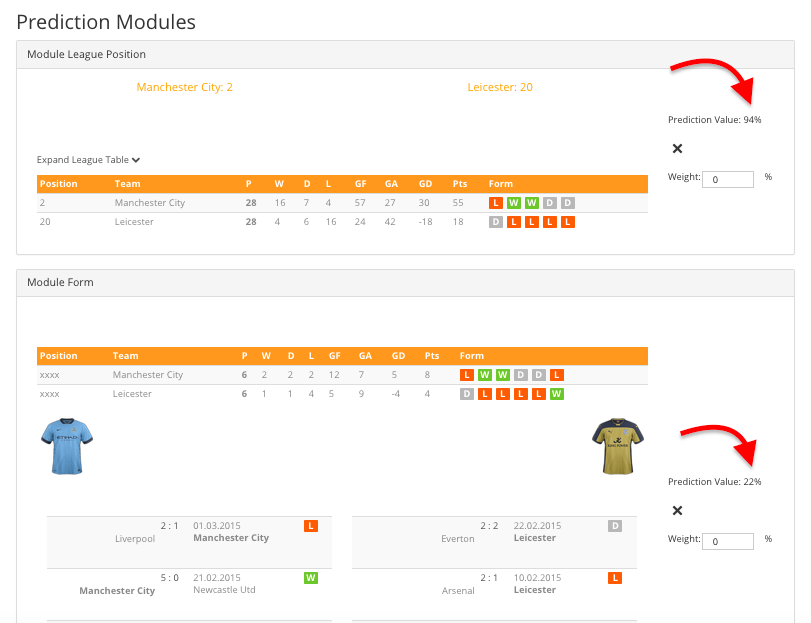
\includegraphics[width=.80\textwidth]{impl/images/predictionValues}
		\caption{Prediction values can be found on the panels for each module.} \label{fig:using: predictionvalues}
	\end{center}
\end{figure}

\subsubsection*{How the prediction values are calculated}
There are quite simple and logical equations behind each of the prediction values. Note that \emph{prediction\_league\_position()}, \emph{prediction\_form()} and \emph{prediction\_homeaway()} functions that hold the calculation code are implemented as properties of a class representing the database model \emph{Match} and therefore can be easily accessed from any part of the code. 

Module League position compares positions in the league table for each of the teams. To calculate the prediction value behind module League Position we first "revert" the league position of each team by subtracting it from the total number of positions in the league, which is 20 for the Premier League. The maximum "reverted" value that may be achieved by each team is 19 (as the top league position is 1). Next, we find the difference between the two obtained values and divide it by the maximum "reverted" value, which is again 19.  Below can be found the equation and the code implementing it.

\begin{equation}
   prediction\_value = \frac{(20-hometeam\_position)-(20-awayteam\_position)}{19}
\end{equation}

\begin{figure}[H]
	\begin{center}
		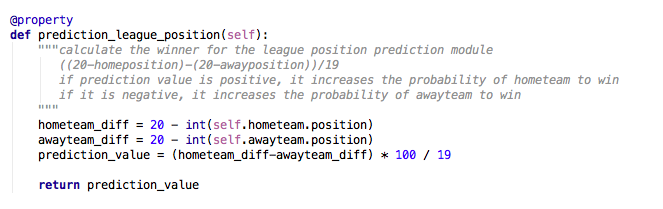
\includegraphics[width=.80\textwidth]{impl/images/predictionLeaguePosition}
		\caption{The calculation behind the prediction value for the module League Position.} \label{fig:using: predictionleagueposition}
	\end{center}
\end{figure}

Module Form takes into consideration team performance in the last 6 games. To calculate the prediction value for the Form module, we need to consider the difference between points achieved by the teams in the last 6 games (this value is taken directly from the league standings table). Obtained difference is then divided by 18, the maximum number of points a team can achieve.

\begin{equation}
   prediction\_value = \frac{(hometeam\_points)-(awayteam\_points)}{18}
\end{equation}


\begin{figure}[H]
	\begin{center}
		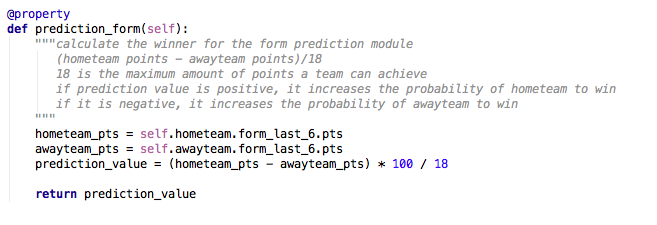
\includegraphics[width=.80\textwidth]{impl/images/predictionForm}
		\caption{The calculation behind the prediction value for the Form module.} \label{fig:using: predictionform}
	\end{center}
\end{figure}

For the Home/Away module we consider the last 6 matches for the home team played \emph{at home} and for the away team played \emph{away}. The equasion behind the prediction value for the module Home/Away is similar to the one above. However, this time we compare points representing \emph{home} performance for the home team and \emph{away} performance for the away team. 

\begin{equation}
   prediction\_value = \frac{(hometeam\_home\_points)-(awayteam\_away\_points)}{18}
\end{equation}

\begin{figure}[H]
	\begin{center}
		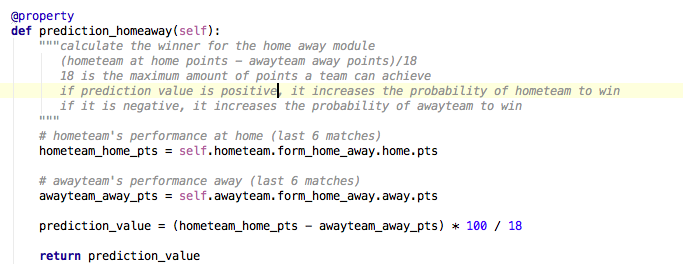
\includegraphics[width=.80\textwidth]{impl/images/predictionHomeAway}
		\caption{The calculation behind the prediction value for the Home/Away module.} \label{fig:using: predictionhomeaway}
	\end{center}
\end{figure}

A simple rule of thumb works for all modules: a positive prediction value represents higher chances for the hometeam to win. The higher the value the higher is the probability of this to happen. On the other hand, a negative value means that the awayteam is more likely to win the match. 

\subsubsection*{How the is the match result predicted}
As already mentioned above, the overall match result is calculated as a weighted average of the prediction values. Application only has to decide which set of weights to use, depending on whether the user provided match specific or user specific settings. Below is an example of how this calculation is performed.

\begin{figure}[H]
	\begin{center}
		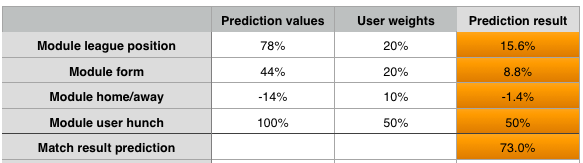
\includegraphics[width=.80\textwidth]{impl/images/overallPredictionCalculation}
		\caption{The table illustrates the calculation behind prediction of match result.} \label{fig:using: overallpredictioncalculation}
	\end{center}
\end{figure}

As it can be seen in the table above, modules' League Position and Form prediction values indicate that the hometeam has strong chances to win the match, as the values are positive (78\% and 44\%). However, the negative value of the module Home/Away implies that there is 14\% probability that the awayteam will be the winner. It is also obvious that the user is favouring the hometeam, as the user hunch prediction value is positive and equals to 100\%. These values are averaged by the user default weights as follows: 

\begin{equation}
   match\_result\_prediction = \frac{78\%*20\% + 44\%*20\% -14\%*10\% + 100\%*50\%}{100\%}
\end{equation}

The overall result is \textbf{78\%}. The high positive value of the obtained value means that the hometeam is very likely to win the match.


\subsection{Played Match View}
\label{subsec:playedmatchview}
User can navigate to this view by clicking the button "View match stats" on a panel representing a match that has already been played. Unlike the \emph{Upcoming Match View}, the \emph{Played Match View} looks the same to the users coming to this page both from their dashboards and from the matches overview page. 

The view contains already familiar match header, prediction statistics and a personalised feedback for the authenticated user. 

\begin{figure}[H]
	\begin{center}
		
\includegraphics[width=.90\textwidth]{impl/images/matchHeader}
		\caption{Played Match View, match header.} \label{fig:matchheader}
	\end{center}
\end{figure}

Prediction statistics block contains information on the betting performance accross the SureThing users population with regards to this match. Stats contain the information on the number of users who saved the match to their dashboards, made a bet on the match, won or lost the bet. 

\begin{figure}[H]
	\begin{center}
		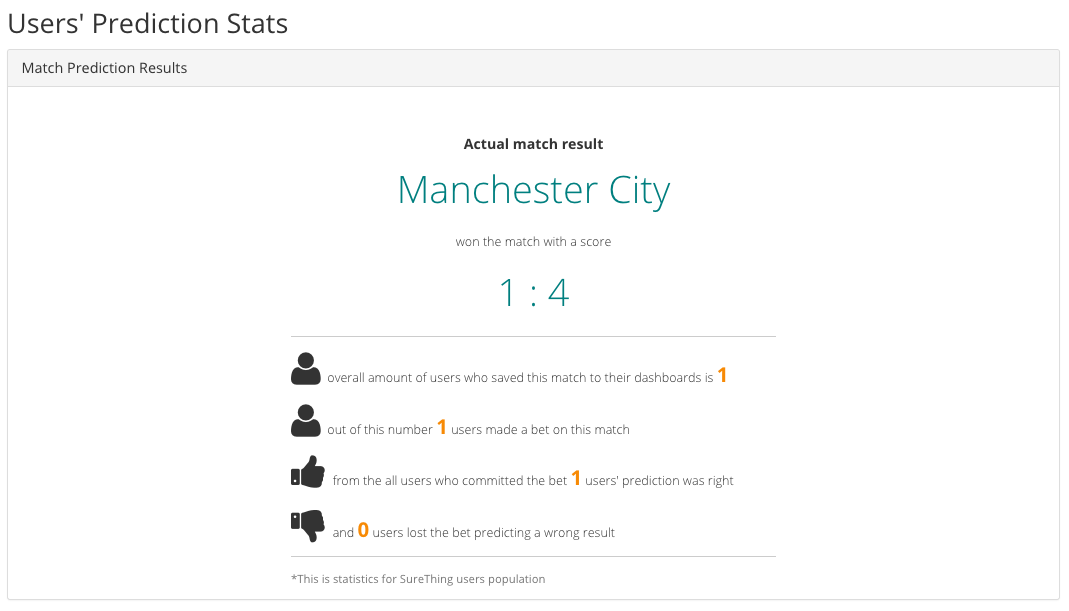
\includegraphics[width=.90\textwidth]{impl/images/predictionStats}
		\caption{Played Match View, users' prediction statistics.} \label{fig:predictionStats}
	\end{center}
\end{figure}

The view also offers a bar chart illustrating a breakdown of user preferences, namely how many users bet on "home", "draw" and "away" result.

\begin{figure}[H]
	\begin{center}
		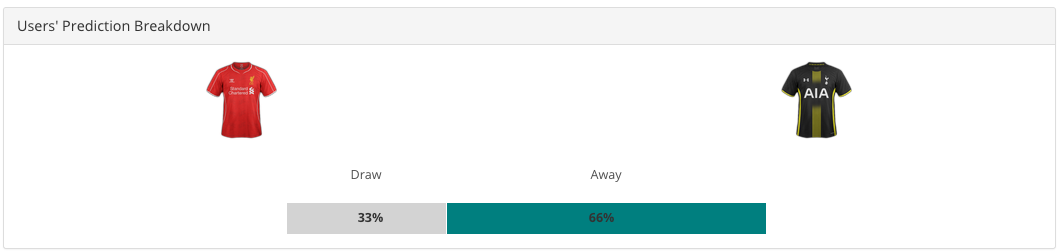
\includegraphics[width=.90\textwidth]{impl/images/predictionBreakdown}
		\caption{Prediction breakdown.} \label{fig:predictionBreakdown}
	\end{center}
\end{figure}

An authenticated user can also view a basic feedback indicating whether this particular user won or lost the bet.

\begin{figure}[H]
	\begin{center}
		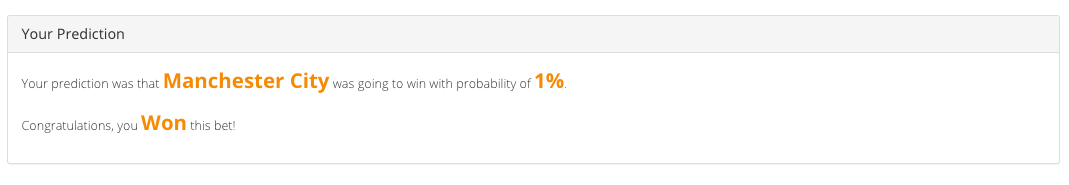
\includegraphics[width=.90\textwidth]{impl/images/feedback}
		\caption{Played Match View, feedback provided for authenticated users.} \label{fig:feedback}
	\end{center}
\end{figure}

\subsubsection*{User journey}
\label{subsec:playedmatchviewuserjourney}
The view is static and does not offer any additional interactions.

\subsection{Dashboard}
\label{subsec:dashboard}
SureThing dashboard is a centralised user space that provides convinient shortcuts to all the important prediction-related pages and tools. Dashboard can be used to store and view matches, change default prediction weights and make bets. It can be navigated to by clicking on item "Dashboard" in the navigation menu of the website, located at the top of the page. On navigating to the dashboard user can see a list of saved matches ordered by date and a \emph{dashboard menu} icon in the top left corner of the view. This is a screenshot of a typical dashboard view (only one match is saved):

\begin{figure}[H]
	\begin{center}
		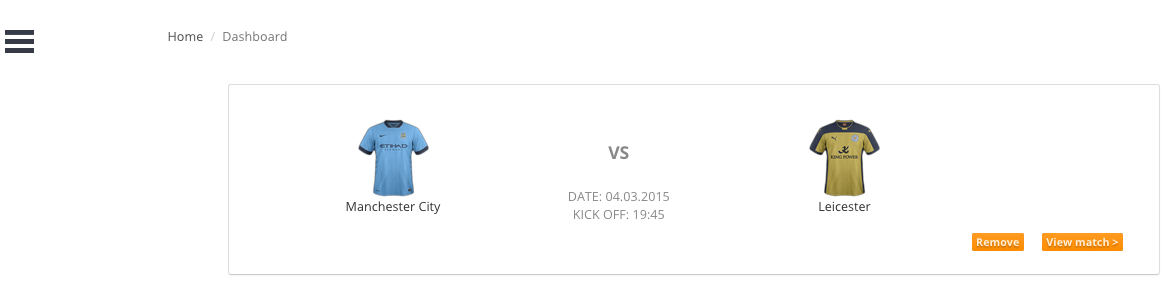
\includegraphics[width=.90\textwidth]{impl/images/typicalDashboard}
		\caption{Dashboard view.} \label{fig:typicaldashboard}
	\end{center}
\end{figure}

Matches that already have been committed by the user have grey background and the predicted winner is highlighted. If the match has already been played, the result of the bet, either "Win" or "Loss" also appears on the match panel.

\begin{figure}[H]
	\begin{center}
		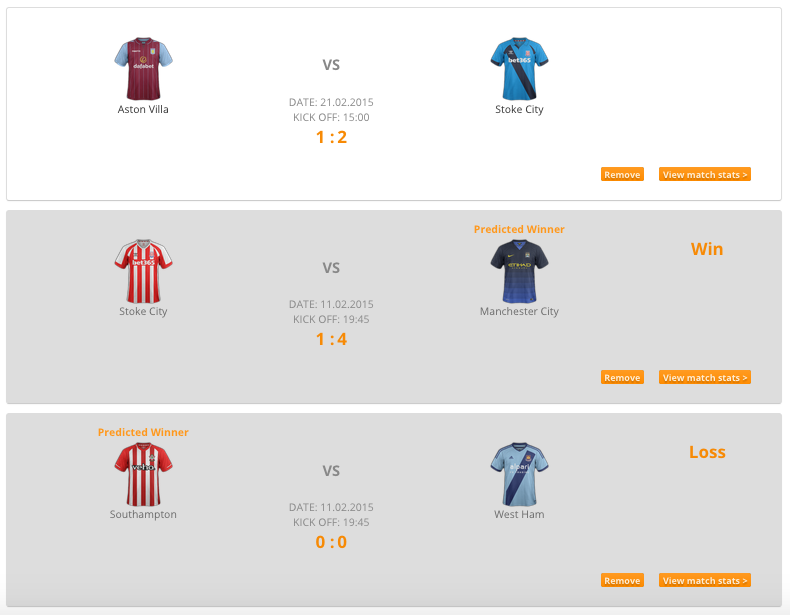
\includegraphics[width=.90\textwidth]{impl/images/dashboardCommittedMatches}
		\caption{An example of a Dashboard View with matches that have been committed and played.} \label{fig:dashboardcommittedmatches}
	\end{center}
\end{figure}

In case user does not have any matches saved, the dashboard looks as follows:

\begin{figure}[H]
	\begin{center}
		
\includegraphics[width=.90\textwidth]{impl/images/noSavedMatches}
		\caption{Dashboard with no saved matches.} \label{fig:using: nosavedmatches}
	\end{center}
\end{figure}

\subsubsection*{User journey}
\label{subsec:dashboarduserjourney}
In the top left corner user can see a small menu icon representing the dashboard menu. Clicking the button opens up the menu containing three items:

\begin{itemize}
	\item{Upcoming Matches. Displays all saved matches that have not been played yet. }
	\item{Archived Matches. Displays all saved matches that have already been played.}
	\item{Prediction Settings. A form that allows the user to set default prediction weights.}
\end{itemize}

A panel containing the dashboard menu slides in and covers part of the page. It can be easily dissmissed by choosing an item from the menu or clicking the "close" icon.

\begin{figure}[H]
	\begin{center}
		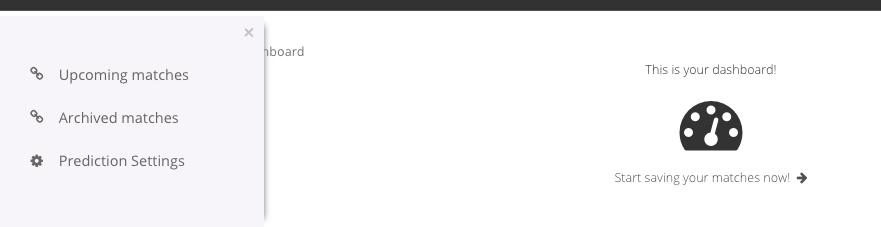
\includegraphics[width=.90\textwidth]{impl/images/dashboardMenu}
		\caption{Dashboard menu.} \label{fig:using: dashboardmenu}
	\end{center}
\end{figure}

If there no saved matches in the dashboard, user can navigate to the main pages containing upcoming events by clicking the link "Start saving your matches now >".

\subsection{Notifications}
\label{subsec:notifications}
This feature represents the one-way communication flow from SureThing to the application user. Every time a match previously commited by the user is finished (from the technical point of view, the match is changing its status to "played"), the application sends users messages notifying them whether their prediction guess was successfull. Such messages contain detailed information about the user prediction, as well as a link to the relevant \emph{Played Match View}.

\begin{figure}[H]
	\begin{center}
		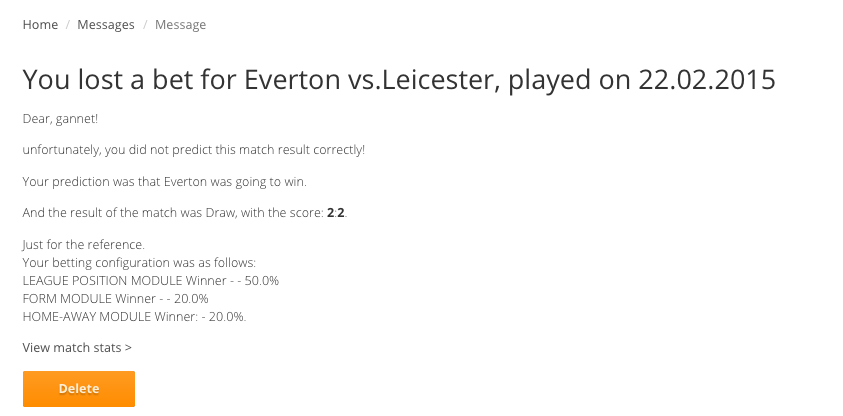
\includegraphics[width=.90\textwidth]{impl/images/message}
		\caption{An example of a message sent to the user.} \label{fig:using: message}
	\end{center}
\end{figure}

\subsubsection*{User journey}
\label{subsec:notificationsuserjourney}
Authenticated user can navigate to the notifications inbox by clicking at the envelope-shaped icon located on the right-hand side of the navigation menu. The orange colour of the icon in the screenshot below indicates that the inbox contains unread messages, otherwise the icon color is grey.

\begin{figure}[H]
	\begin{center}
		
\includegraphics[width=.90\textwidth]{impl/images/navigationMenu}
		\caption{Navigation menu panel with an inbox icon.} \label{fig:using: navigationmenu}
	\end{center}
\end{figure}

On clicking the icon user is taken to the notifications inbox. Unread messages are displayed in bold font.

\begin{figure}[H]
	\begin{center}
		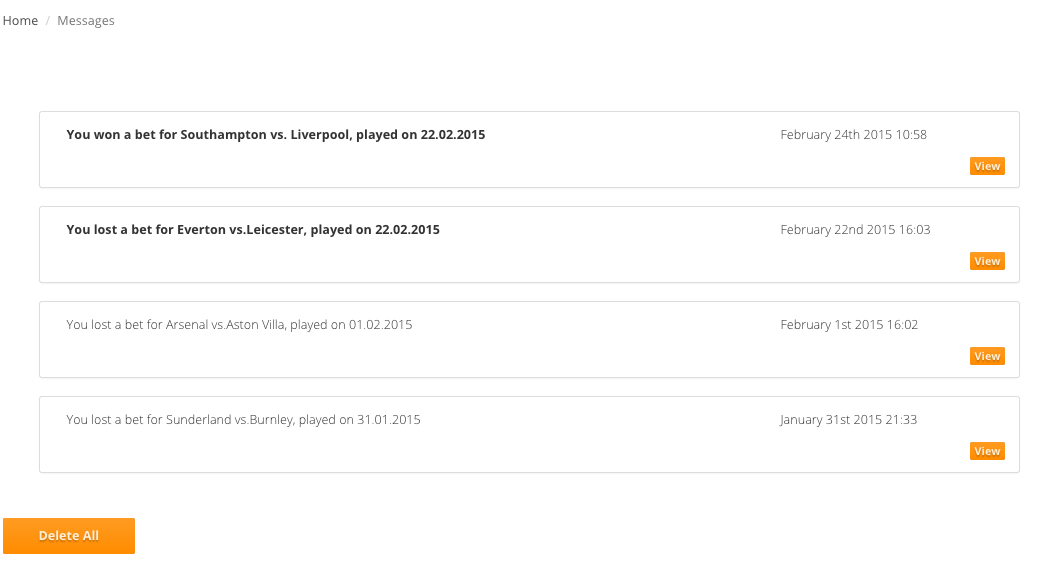
\includegraphics[width=.90\textwidth]{impl/images/inbox}
		\caption{User inbox.} \label{fig:using: inbox}
	\end{center}
\end{figure}

\subsection{Leaderboard}
\label{subsec:leaderboard}
Leaderboard is a view that contains a table capturing betting performance accross the population of the website. This page can be navigated to by clicking a "Leaderboard" entry in the navigation menu of the application. Each line of the Leaderboard table contains the most basic information about application users: usernames, location and their favourite team as well as the betting statistics: games committed, won and lost. The table is ordered by the amount of win points for each user. Thus, the winners are located on the top of the table. 

\begin{figure}[H]
	\begin{center}
		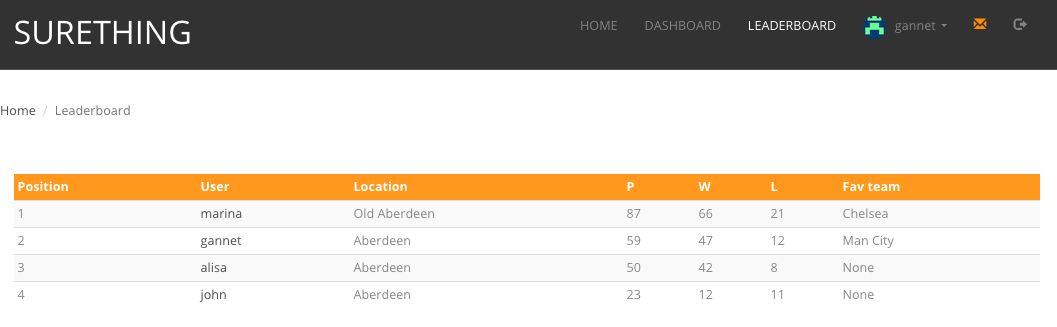
\includegraphics[width=.90\textwidth]{impl/images/leaderboard}
		\caption{Leaderboard.} \label{fig:using: leaderboard}
	\end{center}
\end{figure}

\subsubsection*{User Journey}
\label{subsec:leaderboarduserjourney}
Each username in the table is also a link. Clicking on the username of a user will take us to this user's profile page. Thus, an authenticated user can also view profiles of fellow users.

\section{Application Performance}
\label{sec:applicationperformance}
Performance is a very important aspect of a web application. DEF 

response time 

sockets, threads
multithreading
how I fixed performance on Match.update\_all\_matches
How I measured time

\section{Deploying the Application}
Due to the tight time restrictions the application was not deployed. If it would be deployed, 

Cloud Deployment is the most recent trend in application hosting. The formal name of this technology is Platform as a Service (PaaS).  In the PaaS model, a service provider offers a fully managed platform in which applications can run.
